\section{Simulating a Traffic Sign Recognition AV System}
The system designed for this case study was made to reflect a \acf{AV} and its object detection mechanisms. 
The system used multiple techniques to tackle the inherent issues of the \ac{AV} system, i.e. weakness to perturbed inputs and misclassification of detected objects.
The system's sensors included an overhead, 360$^\circ$ \acf{LiDAR} apparatus, and a single set of front-facing cameras.
Using only front-facing cameras was sufficient to prove the efficacy of this solution, however it is to be noted that \ac{AV} systems generally use cameras facing multiple, different directions, so that the controller can make properly informed decisions.
The architecture of the system used can be seen in Figure~\ref{fig:ssnn}. 

\subsection{Architecture of a Traffic Sign Recognition AV System}
Utilising synchronous semantics~\cite{benveniste2003synchronous}, a \acf{MNN}, containing three other \ac{MNN} ensembles, was created.
A \ac{MNN} is structure containing at least one \acf{SSNN}~\cite{sann} synchronously combined with any number of other functional blocks~\cite{sann}.
Each of the three \ac{MNN} ensembles were used to classify shape, colour and object type of each object being output by the camera.
Each ensemble synchronously combined the outputs of three different convolutional \acp{SSNN}, providing increased prediction accuracy for shape, colour and object type. 
Each \ac{SSNN} was implemented in the synchronous language Esterel~\cite{Esterel}.
Synchronous programming guarantees code that is deterministic, causal and bounded.
Additionally, the calculation of \acf{WCET} and \acf{WCRT} is enabled by using Esterel with C.
These ensembles ran in synchronous concurrency with each other, forming a single, larger \ac{MNN}. 
The outputs of each ensemble were then combined into a batch of outputs forming the \textit{predicted output}.

\begin{figure}[h]
	\centering
	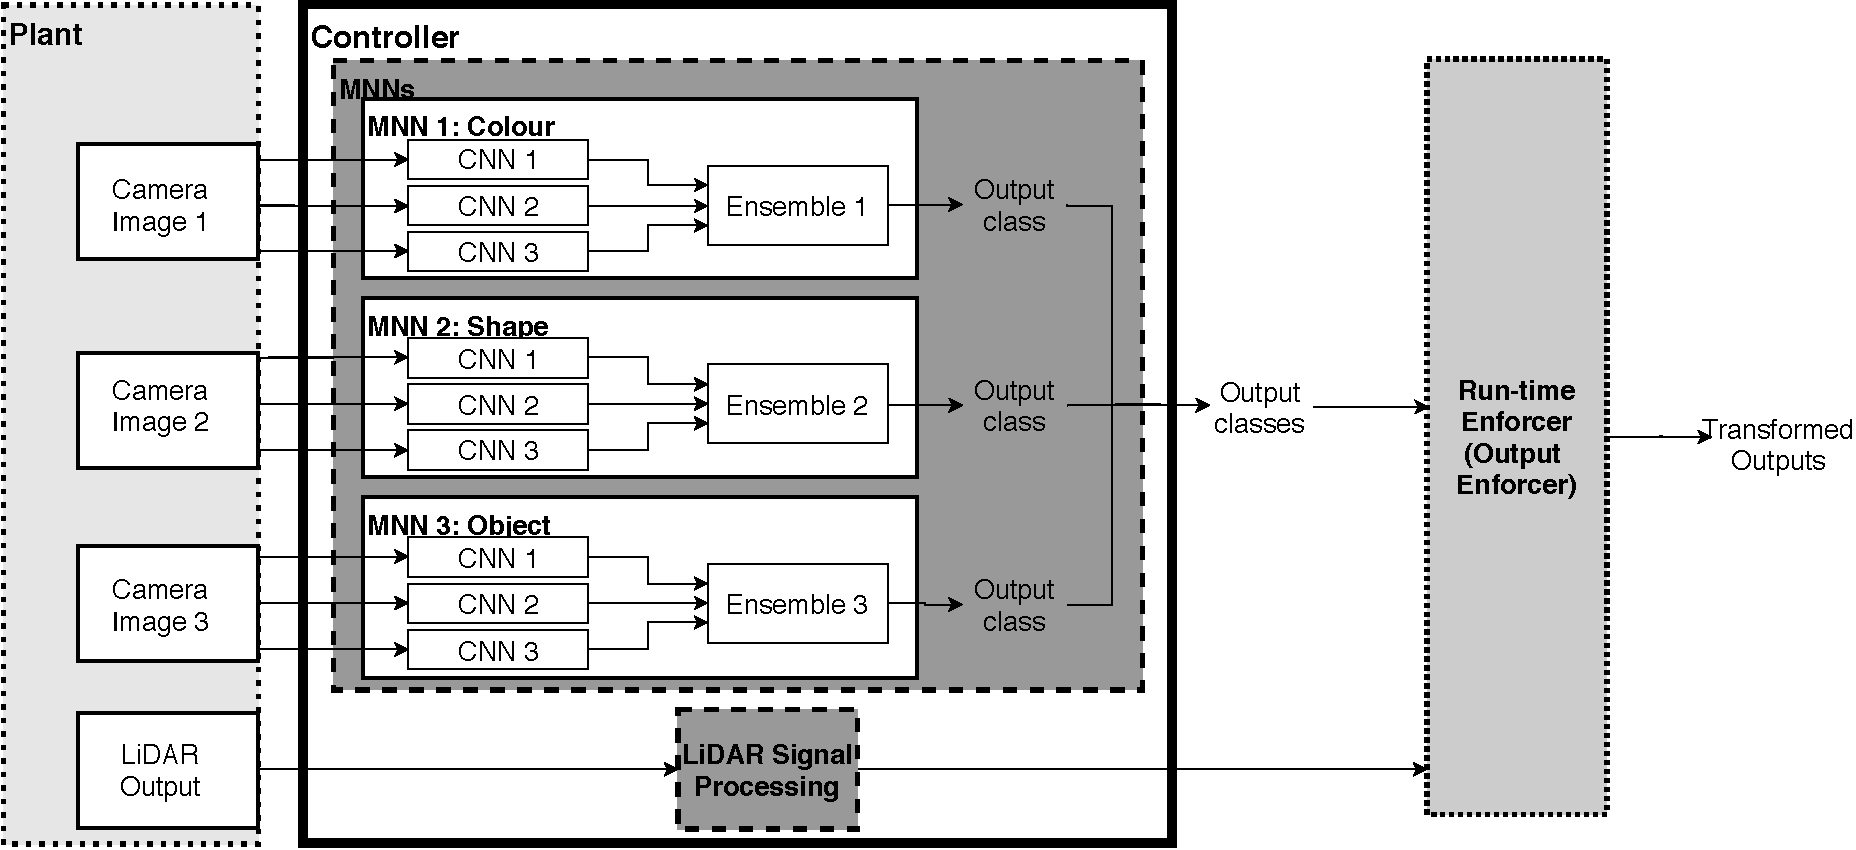
\includegraphics[scale=0.9]{Content/fig/MNN.pdf}
	\caption{Block diagram showing the \acf{MNN} ensemble} \label{fig:mnn}
\end{figure}

\subsection{Sensor Fusion for a Traffic Sign Recognition AV System}
Two sensors were used for the purpose of sensor fusion; \ac{LiDAR} and cameras.
The \ac{LiDAR} controller for this system was accurate 93\% of the time~\cite{lidarFusion}, to closely simulate a system using real \ac{LiDAR}.
The simulated camera outputs consisted of test images from both the \ac{VOC} 2012~\cite{pascal-voc-2012} and \ac{GTSRB}~\cite{Stallkamp2012-gtsrb} datasets, in a combination of people, vehicles and various traffic signs.
The \ac{LiDAR} and camera outputs were handled by different parts of the controller.
The camera outputs were fed into a \ac{MNN} (see Figure~\ref{fig:mnn}) where they were classified by shape, colour and object type.
Sensor fusion happened after classification occurred and was done using an enforcer during runtime.

\subsection{Input Perturbation Safety Policy}
A safety (timed) automata~\ref{recps} was designed to verify predictions made by the \ac{MNN} and ensure utmost safety at all times.
The automata started in a safe state, where control of the vehicle was autonomously handled by the system controller.
If a misclassification was detected, the enforced policy entered an unstable state, still under autonomous control. 
Once enough time passed without further misclassifications, the vehicle entered the safe state again.
However, if another misclassification was detected while unstable, the enforced policy entered a violation state and forced control of the \ac{AV} to the driver.
The vehicle would not enter autonomous mode again until the system was restarted.
A diagram of the enforced policy's safety automaton is shown in Figure~\ref{fig:signrte}.
\begin{figure}[t]
	\centering
	\scalebox{1.3}{

\begin{tikzpicture}[>=stealth',shorten >=1pt,auto,node distance=3 cm, scale = 1, transform shape]

\tikzstyle{accept} = [draw=blue!75,fill=blue!20]
\tikzstyle{violate} = [draw=red!75,fill=red!40, dashed]
\tikzstyle{unstable} = [draw=red!75,fill=red!15]

\node[initial,state, accepting, accept] (A) {$q_{auto}$};
\node[state, unstable] (B) [right of=A] {$q_{unstable}$};
\node[state, violate]         (C) [below of=B, xshift=-1.5cm]  {$q_v$};

\path[->] 
		(A) edge [loop above]       node [above]  
		{
			\scriptsize$\let\scriptstyle\textstyle\substack{\overline{M}}$
		} (A)
		
		(A) edge [bend left]		node [below]  
		{
			\scriptsize$\let\scriptstyle\textstyle\substack{
				M,~\\~
				t~:=~0~
			}$
		} (B)
	
		(B) edge [loop above]		node [above]  
		{
			\scriptsize$\let\scriptstyle\textstyle\substack{t~<~3~\&~\\~~\overline{M}}$
		} (B)
	
		(B) edge [bend left]		node [right]  
		{
			\scriptsize$\let\scriptstyle\textstyle\substack{M}$
		} (C)
	
		(B) edge [bend left]		node [below]  
		{
			\scriptsize$\let\scriptstyle\textstyle\substack{t~>=~3~\&\\~\overline{M}}$
		} (A)
	
		(C) edge [loop below] node [below]
		{
			\scriptsize$\sum$
		}(C)
		;

\end{tikzpicture}}
	\begin{itemize}
		\item $P$: Misclassification of a person.
		\item $V$: Misclassification of a vehicle.
		\item $N$: Classification of an object when there is nothing.
		\item $S$: Misclassification of a traffic sign.
		\item $C$: Confidence rating of the \ac{SSNN} classification.
		\item $t$: Timer for the unstable state.
	\end{itemize}
	
	\caption{Enforcer policy for the \acf{AV} prediction system}
	\label{fig:signrte}
\end{figure}

\subsection{Runtime Enforcer for a Traffic Sign Recognition AV System}
The system controller was encapsulated by a run-time enforcer~\cite{recps} that used sensor fusion to check for misclassifications made by the \ac{MNN}.
This type of run-time enforcement, where neither the inputs nor outputs of the sensors or controller are enforced, has been termed as \textit{run-time verification}.
\textit{Run-time verification} refers to the verification of system parameters during run-time, while ensuring that the system is aware of any failed guards in the enforced policy.

\begin{figure}[t]
	\centering
	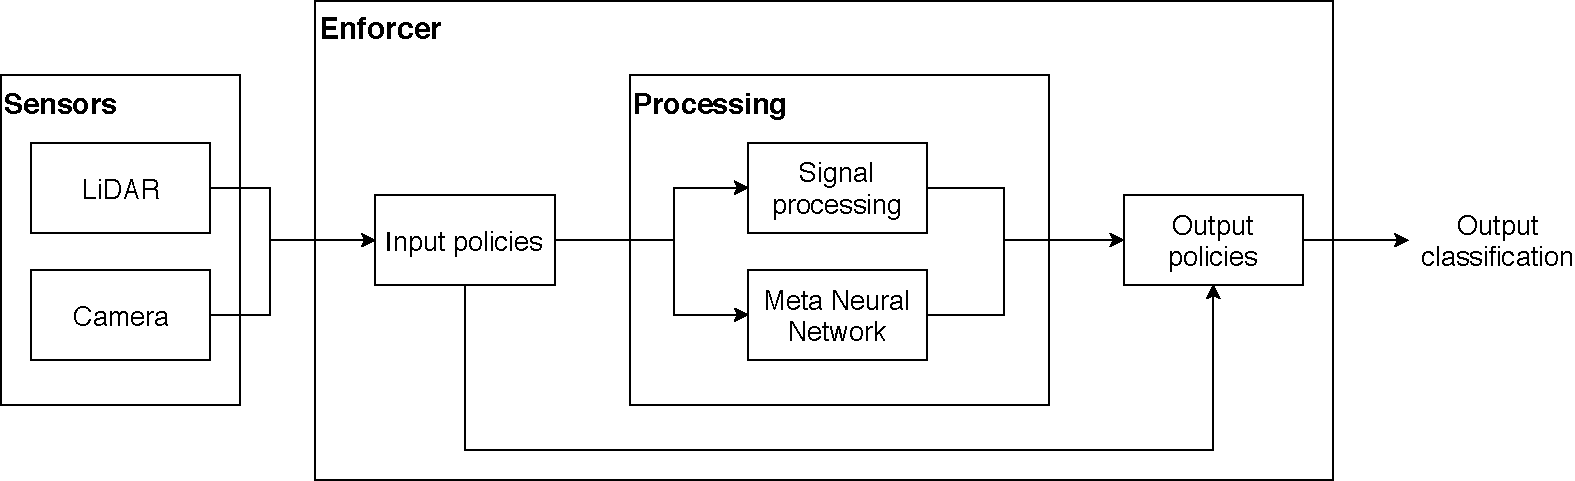
\includegraphics[scale=0.6]{Content/fig/SSNN.pdf}
	\caption{Block diagram showing the \acf{AV} system with enforcer}
	\label{fig:ssnn}
\end{figure}






















